\documentclass[12pt,a4paper,oneside]{report}

% ==============================================================================
% PACKAGES AND STYLING (MATCHING SRM UNIVERSITY-AP B.TECH FORMAT)
% ==============================================================================
\usepackage[utf8]{inputenc}
\usepackage[top=0.85in, bottom=0.85in, left=1.0in, right=1.0in]{geometry}
\usepackage{setspace}
\setstretch{1.12}

\usepackage{amsmath,amssymb,amsfonts}
\usepackage{graphicx}
\graphicspath{{./}{report/}{../report/}}
\usepackage{booktabs}
\usepackage{tabularx}
\usepackage{array}
\usepackage{float}
\usepackage{xcolor}
\usepackage{listings}
\usepackage{fancyhdr}
\usepackage{titlesec}
\usepackage{cite}
\usepackage{enumitem}
\usepackage{microtype}
\usepackage{tikz}
\usetikzlibrary{shapes.geometric, arrows, positioning, fit, backgrounds, calc}

% Palette
\definecolor{primarynavy}{RGB}{15, 23, 42}
\definecolor{accentblue}{RGB}{2, 132, 199}
\definecolor{bordergray}{RGB}{203, 213, 225}
\definecolor{codebg}{RGB}{248, 250, 252}
\definecolor{keywordblue}{RGB}{0, 51, 153}
\definecolor{stringgreen}{RGB}{0, 128, 0}
\definecolor{commentgray}{RGB}{100, 116, 139}

\usepackage[colorlinks=true,linkcolor=primarynavy,citecolor=primarynavy,urlcolor=accentblue,bookmarks=true,bookmarksnumbered=true]{hyperref}
\usepackage{url}

% Listings setup
\lstdefinestyle{JavaStyle}{
    backgroundcolor=\color{codebg},
    basicstyle=\ttfamily\scriptsize,
    breaklines=true,
    captionpos=b,
    commentstyle=\color{commentgray}\itshape,
    frame=single,
    framerule=0.4pt,
    rulecolor=\color{bordergray},
    keywordstyle=\color{keywordblue}\bfseries,
    language=Java,
    numbers=left,
    numbersep=5pt,
    numberstyle=\tiny\color{commentgray},
    showstringspaces=false,
    stringstyle=\color{stringgreen},
    tabsize=4,
    xleftmargin=0.8em,
    framexleftmargin=0.8em
}

\lstdefinestyle{SqlStyle}{
    backgroundcolor=\color{codebg},
    basicstyle=\ttfamily\scriptsize,
    breaklines=true,
    frame=single,
    framerule=0.4pt,
    rulecolor=\color{bordergray},
    keywordstyle=\color{keywordblue}\bfseries,
    language=SQL,
    numbers=left,
    numbersep=5pt,
    numberstyle=\tiny\color{commentgray},
    stringstyle=\color{stringgreen},
    tabsize=4,
    xleftmargin=0.8em,
    framexleftmargin=0.8em
}

% Header and Footer
\pagestyle{fancy}
\fancyhf{}
\fancyfoot[C]{\thepage}
\renewcommand{\headrulewidth}{0pt}
\renewcommand{\footrulewidth}{0pt}

% Chapter formatting tuned to fit strictly within 18 pages total
\titleformat{\chapter}[display]
  {\normalfont\Large\bfseries}
  {\chaptertitlename\ \thechapter}{3pt}{\LARGE}
\titlespacing*{\chapter}{0pt}{4pt}{10pt}
\titlespacing*{\section}{0pt}{7pt}{2pt}
\titlespacing*{\subsection}{0pt}{5pt}{2pt}
\setcounter{tocdepth}{1}

% ==============================================================================
% DOCUMENT STARTS
% ==============================================================================
\begin{document}

% ------------------------------------------------------------------------------
% PAGE 1: TITLE PAGE
% ------------------------------------------------------------------------------
\begin{titlepage}
    \begin{center}
        \vspace*{0.1cm}
        {\LARGE \textbf{ClinicQueue}}\\[0.25cm]
        {\large \textbf{Robust Offline-First Hospital Outpatient Queue Management System Using JavaFX, Transactional JDBC, and Embedded SQLite}}\\[0.55cm]

        {\large \textbf{A PROJECT REPORT}}\\[0.15cm]
        {\normalsize Submitted in partial fulfilment of the requirements for the award of the degree of}\\[0.25cm]

        {\Large \textbf{Bachelor of Technology}}\\[0.15cm]
        {\large \textbf{in COMPUTER SCIENCE AND ENGINEERING}}\\[0.1cm]
        {\normalsize \textbf{(Specialization in Artificial Intelligence and Machine Learning)}}\\[0.45cm]

        \textbf{Submitted by}\\[0.15cm]
        {\textbf{Puvaladas Sai Vaibhav} \hspace{0.5cm} Registration No.: AP25110071052}\\[0.08cm]
        {\textbf{Parth Gupta} \hspace{1.7cm} Registration No.: AP25110071425}\\[0.08cm]
        {\textbf{Aishwarya P} \hspace{1.5cm} Registration No.: AP25110071118}\\[0.08cm]
        {\textbf{Lasya} \hspace{2.4cm} Registration No.: AP25110070394}\\[0.08cm]
        {\textbf{Dhanvin Sinha} \hspace{1.3cm} Registration No.: AP25110070187}\\[0.45cm]

        \textbf{Submitted to}\\[0.15cm]
        {\Large \textbf{Dr. Tirthankar Sengupta}}\\[0.4cm]

        % SRM University-AP Official Emblem
        \IfFileExists{srm_logo.png}{%
            
\includegraphics[width=3.0cm]{srm_logo.png}\\[0.35cm]
        }{%
            \IfFileExists{srm_logo.jpg}{%
                
\includegraphics[width=3.0cm]{srm_logo.jpg}\\[0.35cm]
            }{%
                % Safe vector fallback if no external image files exist
                
\begin{tikzpicture}
                    % Outer boundary circles
                    \draw[thick, color=primarynavy] (0,0) circle (1.35cm);
                    \draw[double, thick, color=primarynavy] (0,0) circle (1.2cm);
                    
                    % Typography
                    \node at (0, 0.85) {\scriptsize \textbf{SRM UNIVERSITY AP}};
                    \node at (0, -0.85) {\tiny \textbf{ANDHRA PRADESH}};
                    \node at (0, 0.28) {\footnotesize \textbf{LEARN $\cdot$ LEAP $\cdot$ LEAD}};
                    
                    % Vector representation of the inner crest (No file dependency)
                    \draw[thick, fill=primarynavy!10, draw=primarynavy] (0,-0.22) circle (0.38cm);
                    \foreach \a in {0,45,...,315} {
                        \draw[thick, color=primarynavy] (0,-0.22) ++(\a:0.38cm) -- ++(\a:0.08cm);
                    }
                    \node at (0, -0.22) {\tiny\color{primarynavy}\textbf{SRM}};
                \end{tikzpicture}\\[0.35cm]
            }%
        }
        

        {\large \textbf{Department of Computer Science and Engineering}}\\[0.08cm]
        {\large \textbf{SRM University--AP}}\\[0.08cm]
        {\normalsize Neerukonda, Mangalagiri, Andhra Pradesh -- 522240, India}\\[0.25cm]

        {\normalsize \textbf{Official GitHub Repository:}}\\[0.08cm]
        {\normalsize \url{https://github.com/vaibhavpuvaladas-byte/ClinicQueue}}\\[0.25cm]
        {\large \textbf{2026}}
    \end{center}
\end{titlepage}

% ------------------------------------------------------------------------------
% PRELIMINARY PAGES (ROMAN NUMBERING)
% ------------------------------------------------------------------------------
\pagenumbering{roman}
\setcounter{page}{1}

% ------------------------------------------------------------------------------
% CERTIFICATE (PAGE i)
% ------------------------------------------------------------------------------
\newpage
\begin{center}
    \vspace*{0.2cm}
    {\Huge \textbf{CERTIFICATE}}\\[0.6cm]
\end{center}

\noindent
This is to certify that the project report entitled \textbf{“ClinicQueue: Robust Offline-First Hospital Outpatient Queue Management System Using JavaFX, Transactional JDBC, and Embedded SQLite”}, submitted by \textbf{Puvaladas Sai Vaibhav} (Registration No. \textbf{AP25110071052}), \textbf{Parth Gupta} (Registration No. \textbf{AP25110071425}), \textbf{Aishwarya P} (Registration No. \textbf{AP25110071118}), \textbf{Lasya} (Registration No. \textbf{AP25110070394}), and \textbf{Dhanvin Sinha} (Registration No. \textbf{AP25110070187}), in partial fulfillment of the requirements for the award of the degree of \textbf{Bachelor of Technology in Computer Science and Engineering (Specialization in Artificial Intelligence and Machine Learning)} at \textbf{SRM University--AP}, is a bonafide record of the project work carried out under my supervision.

\vspace{0.3cm}
\noindent
The work presented in this report has not been submitted, either in whole or in part, for the award of any other degree or diploma to the best of our knowledge.

\vspace{2.5cm}

\noindent
\begin{tabularx}{\textwidth}{X r}
\rule{6.0cm}{0.4pt} & \rule{6.0cm}{0.4pt} \\
\textbf{Dr. Tirthankar Sengupta, Ph.D.}  \\
Project Supervisor \& Associate Professor & Head of the Department \\
Dept. of Computer Science \& Engineering & Dept. of Computer Science \& Engineering \\
SRM University--AP & SRM University--AP \\
\end{tabularx}

\vspace{1.2cm}
\noindent
Place: Neerukonda, Andhra Pradesh\\
Date: 9 November 2026

% ------------------------------------------------------------------------------
% ACKNOWLEDGEMENT & TEAM ROLES (PAGE ii)
% ------------------------------------------------------------------------------
\newpage
\begin{center}
    \vspace*{0.2cm}
    {\Huge \textbf{ACKNOWLEDGEMENT}}\\[0.6cm]
\end{center}

\noindent
We express our deepest gratitude to our project supervisor and course instructor, \textbf{Dr. Tirthankar Sengupta}, Department of Computer Science and Engineering, SRM University--AP, for his continuous guidance, rigorous architectural critiques, and supportive reviews throughout the development of ClinicQueue.

\vspace{0.3cm}
\noindent
\textbf{Team Member Roles and Specialized Responsibilities:}
\vspace{0.15cm}

\begin{table}[H]
\centering
\small
\begin{tabularx}{\textwidth}{p{4.2cm} p{2.8cm} X}
\toprule
\textbf{Student Name} & \textbf{Registration No.} & \textbf{Specialized Role \& Contribution} \\
\midrule
Puvaladas Sai Vaibhav & AP25110071052 & System Architecture, SQLite Schema DDL, JDBC Transaction Boundaries \\
Parth Gupta & AP25110071425 & Business Logic Services, Queue State Machine, Domain Invariant Enforcement \\
Aishwarya P & AP25110071118 & Presentation Layer Architecture, JavaFX Layout Views, Visual Styling \\
Lasya & AP25110070394 & Queue Board Controller, Search/Filter Streams, Wait-Time Algorithms \\
Dhanvin Sinha & AP25110070187 & QA Automation, Headless JUnit 5 Suites, Technical Documentation \\
\bottomrule
\end{tabularx}
\end{table}

\vspace{0.6cm}
\noindent
\begin{tabularx}{\textwidth}{X r}
 & \textbf{Puvaladas Sai Vaibhav} \\
 & \textbf{Parth Gupta} \\
 & \textbf{Aishwarya P} \\
 & \textbf{Lasya} \\
 & \textbf{Dhanvin Sinha} \\
\end{tabularx}

% ------------------------------------------------------------------------------
% ABSTRACT (PAGE iii)
% ------------------------------------------------------------------------------
\newpage
\begin{center}
    \vspace*{0.2cm}
    {\Huge \textbf{ABSTRACT}}\\[0.6cm]
\end{center}

\noindent
Outpatient Departments (OPD) in hospitals and polyclinics frequently encounter severe operational bottlenecks due to chaotic patient arrivals, uncoordinated paper-based token slips, and verbal callouts. While modern enterprise cloud Hospital Information Systems (HIS) offer digital tracking, their strict dependence on continuous high-speed internet makes them vulnerable to connectivity blackouts in peripheral and edge healthcare clinics.

\vspace{0.25cm}
\noindent
To resolve these operational challenges, this project presents \textbf{ClinicQueue}, an offline-first desktop queue management system engineered in Java 21 LTS using JavaFX, transactional JDBC, and an embedded SQLite database engine. ClinicQueue eliminates queue jumping by generating structured, daily sequential tokens formatted as \texttt{D\{doctorId\}-\{date\}-\{sequence\}} governed by database-enforced composite uniqueness constraints.

\vspace{0.25cm}
\noindent
The consultation lifecycle is modeled as a deterministic 4-state Finite State Machine (\texttt{WAITING} $\rightarrow$ \texttt{IN\_CONSULTATION} $\rightarrow$ \texttt{COMPLETED}; \texttt{WAITING} $\rightarrow$ \texttt{CANCELLED}). Clinical chamber crowding is strictly prevented through an invariant guard rule that blocks a physician from calling a patient while an active consultation is in progress. A dynamic wait-time estimation engine computes approximate wait durations based on queue position multiplied by average consultation times ($N \times 10$ minutes).

\vspace{0.25cm}
\noindent
ClinicQueue has been refactored into a high-performance codebase of 1,099 core Java lines across 23 classes, achieving 100\% automated pass rates across 15 functional acceptance requirements under JUnit 5, zero sequence collisions under concurrent stress, sub-5ms query latencies, and total offline persistence. The open-source code and build configuration are maintained at: \url{https://github.com/vaibhavpuvaladas-byte/ClinicQueue}.

\vspace{0.35cm}
\noindent
\textbf{Keywords:} Healthcare Informatics, Queue Management System, JavaFX, SQLite, Finite State Machine, ACID Transactions, Offline-First Desktop Application.

% ------------------------------------------------------------------------------
% CONTENTS (PAGE iv)
% ------------------------------------------------------------------------------
\newpage
\tableofcontents

% ------------------------------------------------------------------------------
% LIST OF FIGURES, TABLES & ABBREVIATIONS (PAGE v)
% ------------------------------------------------------------------------------
\newpage
\addcontentsline{toc}{chapter}{LIST OF FIGURES AND TABLES}
\begin{center}
    {\Large \textbf{LIST OF FIGURES AND TABLES}}\\[0.25cm]
\end{center}

\noindent
\textbf{List of Figures}
\vspace{0.1cm}

\noindent
\begin{tabularx}{\textwidth}{p{1.2cm} X r}
4.1 & High-level layered architecture of ClinicQueue & 5 \\
4.2 & Deterministic visit state transition diagram & 6 \\
\end{tabularx}

\vspace{0.3cm}
\noindent
\textbf{List of Tables}
\vspace{0.1cm}

\noindent
\begin{tabularx}{\textwidth}{p{1.2cm} X r}
2.1 & Comparison of relevant outpatient queue management approaches & 2 \\
3.1 & Software and development environment requirements & 4 \\
4.1 & Major software modules and package responsibilities & 5 \\
6.1 & Functional test matrix and representative test cases & 9 \\
6.2 & Experimental performance benchmarks and metrics & 10 \\
\end{tabularx}

\vspace{0.4cm}
\addcontentsline{toc}{chapter}{LIST OF ABBREVIATIONS}
\begin{center}
    {\Large \textbf{LIST OF ABBREVIATIONS}}\\[0.2cm]
\end{center}

\noindent
\small
\begin{tabularx}{\textwidth}{p{2.2cm} X p{2.2cm} X}
ACID & Atomicity, Consistency, Isolation, Durability & JDBC & Java Database Connectivity \\
API & Application Programming Interface & JDK & Java Development Kit \\
CSS & Cascading Style Sheets & JVM & Java Virtual Machine \\
DAO & Data Access Object & OPD & Outpatient Department \\
DTO & Data Transfer Object & PII & Personally Identifiable Information \\
FIFO & First-In, First-Out & RDBMS & Relational Database Management System \\
FSM & Finite State Machine & SoC & Separation of Concerns \\
GUI & Graphical User Interface & SQL & Structured Query Language \\
HIS & Hospital Information System & UI & User Interface \\
\end{tabularx}

% ------------------------------------------------------------------------------
% MAIN CHAPTERS (ARABIC PAGE NUMBERING)
% ------------------------------------------------------------------------------
\newpage
\pagenumbering{arabic}
\setcounter{page}{1}

% ==============================================================================
% CHAPTER 1: INTRODUCTION (EXACTLY 1 PAGE)
% ==============================================================================
\chapter{INTRODUCTION}

\section{Project Background and Motivation}
Healthcare Outpatient Departments (OPD) serve as the primary public point of contact, managing daily influxes of scheduled and walk-in visitors. Historically, outpatient triage has relied on manual ledgers or paper tickets, leading to waiting hall overcrowding, patient anxiety, and disputes. Conversely, commercial cloud Hospital Information Systems (HIS) require continuous internet, failing completely during peripheral clinic network drops. \textbf{ClinicQueue} resolves these challenges as an offline-first Java desktop application combining JavaFX 21 LTS, transactional JDBC, and an embedded SQLite database engine.

\section{Problem Statement and Objectives}
The project eliminates clinic waiting room disorganization by automating patient intake, generating unique sequential daily tokens, and enforcing single-patient consultation invariants. The core objectives are:
\begin{enumerate}[leftmargin=0.7cm, itemsep=0.5pt]
    \item Develop an offline-first desktop queue management system using JavaFX and SQLite.
    \item Implement rapid patient registration with real-time whitespace trimming and phone validation.
    \item Generate structured sequential tokens formatted as \texttt{D\{doctorId\}-\{date\}-\{sequence\}}.
    \item Enforce a 4-state Finite State Machine (\texttt{WAITING}, \texttt{IN\_CONSULTATION}, \texttt{COMPLETED}, \texttt{CANCELLED}).
    \item Prevent doctor chamber crowding by blocking calls when another consultation is active.
    \item Calculate dynamic wait-time estimations based on queue depth ($N \times 10$ minutes).
    \item Validate transaction safety and sub-5ms query performance via automated JUnit 5 tests.
\end{enumerate}

\section{Project Scope and Contributions}
ClinicQueue targets single-workstation clinic desks and doctor chambers, providing full local persistence (\texttt{clinicqueue.db}) without cloud dependencies. Key contributions include an atomic composite-key token allocator, single-consultation invariant guards, a streamlined 1,099-line Java codebase, and 100\% pass rates across 15 acceptance criteria.

\section{Official Source Code Repository}
The production codebase, schema migrations, and test suites are maintained on GitHub:
\begin{center}
\textbf{Official GitHub Repository:} \url{https://github.com/vaibhavpuvaladas-byte/ClinicQueue}
\end{center}

\section{Report Organisation}
Chapter 2 reviews related queuing literature. Chapter 3 analyzes system requirements. Chapter 4 presents architecture and database design. Chapter 5 details implementation. Chapter 6 discusses experimental test results. Chapter 7 concludes the report.

% ==============================================================================
% CHAPTER 2: RELATED WORK AND LITERATURE REVIEW (EXACTLY 1 PAGE)
% ==============================================================================
\chapter{RELATED WORK AND LITERATURE REVIEW}

\section{Queuing Theory in Healthcare Operations}
Mathematical queuing analysis in healthcare began with Bailey's study on outpatient appointment systems \cite{bailey1952study}. Outpatient clinics are modeled as stochastic queues where arrival rate $\lambda$ and doctor consultation rate $\mu$ govern congestion. By Little's Law \cite{little1961proof}:
\begin{equation}
    \bar{L} = \lambda \cdot \bar{W}
\end{equation}
where $\bar{L}$ is the mean queue length and $\bar{W}$ is the mean waiting time. Cayirli and Veral \cite{cayirli2003outpatient} proved that communicating estimated wait times substantially lowers perceived patient anxiety and waiting room stress.

\section{Hospital Outpatient Bottlenecks and Digital Triage}
Acheampong et al. \cite{acheampong2019queuing} established that physical waiting room crowding elevates nosocomial transmission risks. Digital queue boards restore order by enforcing strict First-In, First-Out (FIFO) queue discipline.

\section{Comparative Analysis of Prevailing Approaches}
Table 2.1 contrasts ClinicQueue with existing queue management solutions:

\begin{table}[H]
\centering
\small
\begin{tabularx}{\textwidth}{p{3.2cm} X X}
\toprule
\textbf{Approach} & \textbf{Primary Operational Mechanism} & \textbf{Critical Limitation} \\
\midrule
Manual Paper Slips & Physical printed or handwritten slips & Prone to loss, queue jumping, zero wait transparency. \\
Cloud SaaS Systems & Remote booking via internet & Total shutdown during internet outages; recurring fees. \\
Enterprise HIS / EHR & Comprehensive electronic hospital records & High capital cost, server setup overhead, complexity. \\
\textbf{ClinicQueue (Ours)} & \textbf{Offline-first JavaFX + SQLite persistence} & \textbf{Single workstation focus in initial release.} \\
\bottomrule
\end{tabularx}
\caption{Comparison of relevant outpatient queue management approaches}
\end{table}

\section{Research Gap and Project Positioning}
Existing literature demonstrates the need for queue discipline but highlights the operational fragility of cloud architectures in edge clinics. ClinicQueue bridges this gap by delivering an offline-first desktop solution that guarantees ACID token integrity and clinical chamber invariants without external server dependencies.

% ==============================================================================
% CHAPTER 3: SYSTEM ANALYSIS AND REQUIREMENTS (EXACTLY 2 PAGES)
% ==============================================================================
\chapter{SYSTEM ANALYSIS AND REQUIREMENTS}

\section{Existing System vs. Proposed System}
Conventional clinic waiting rooms rely on manual sign-up sheets or verbal callouts, resulting in disorder, lack of wait-time awareness, and physician interruptions. ClinicQueue replaces this with an integrated desktop application. Staff enter patient information, select consulting doctors, and generate atomic tokens; the real-time queue board displays patients in FIFO order, shows dynamic wait times, and enforces single active consultations.

\section{Functional Requirements}
\begin{itemize}[leftmargin=1.2cm, itemsep=0.5pt]
    \item[\textbf{FR1.}] Register patients with full name and optional contact phone number.
    \item[\textbf{FR2.}] Validate patient names as non-null and non-blank with automated whitespace trimming.
    \item[\textbf{FR3.}] Validate that supplied contact numbers contain at least 7 numerical digits.
    \item[\textbf{FR4.}] Allocate sequential daily tokens formatted as \texttt{D\{doctorId\}-\{date\}-\{sequence\}}.
    \item[\textbf{FR5.}] Guarantee token uniqueness through composite constraints \texttt{UNIQUE(doctor\_id, visit\_date, token\_sequence)}.
    \item[\textbf{FR6.}] Enforce visit lifecycle states: \texttt{WAITING}, \texttt{IN\_CONSULTATION}, \texttt{COMPLETED}, \texttt{CANCELLED}.
    \item[\textbf{FR7.}] Select the oldest waiting patient in strict FIFO order on ``Call Next''.
    \item[\textbf{FR8.}] Prevent a doctor from summoning a patient while an ongoing consultation is active.
    \item[\textbf{FR9.}] Permit completion only for visits currently marked \texttt{IN\_CONSULTATION}.
    \item[\textbf{FR10.}] Restrict cancellation strictly to \texttt{WAITING} visits, requiring confirmation.
    \item[\textbf{FR11.}] Calculate approximate wait times as $(P-1) \times 10$ minutes based on queue position.
    \item[\textbf{FR12.}] Display live aggregated statistics: Total, Waiting, In Consultation, and Completed.
    \item[\textbf{FR13.}] Provide live search and filtering by consulting doctor, visit status, and patient name.
    \item[\textbf{FR14.}] Persist all relational records locally in SQLite with foreign key enforcement.
    \item[\textbf{FR15.}] Offer a confirmed one-click database reset and demonstration re-seed utility.
\end{itemize}

\section{Non-Functional Requirements}
\begin{itemize}[leftmargin=0.8cm, itemsep=0.5pt]
    \item \textbf{Security:} Parameterized \texttt{PreparedStatement} queries prevent SQL injection; minimal PII display.
    \item \textbf{Reliability:} Automatic rollback on SQL failure ensuring zero orphaned patient records.
    \item \textbf{Usability:} Responsive JavaFX GUI with distinct modal alerts and color-coded status chips.
    \item \textbf{Portability:} Standard Java 21 LTS managed via Apache Maven, executable on Windows, Linux, and macOS.
    \item \textbf{Offline Autonomy:} Zero runtime dependencies on cloud services or internet connections.
\end{itemize}

\section{Hardware and Software Requirements}
Table 3.1 specifies the software and environment requirements:

\begin{table}[H]
\centering
\small
\begin{tabularx}{\textwidth}{p{4.2cm} X}
\toprule
\textbf{Requirement Item} & \textbf{Specification / Tool} \\
\midrule
Operating System & Desktop OS supporting JavaFX (Windows 10/11, Ubuntu 20.04+, macOS 12+) \\
Programming Language & Java (JDK 17 or JDK 21 LTS) \\
User Interface Framework & JavaFX 21.0.2 / OpenJFX Controls \\
Build \& Dependency Tool & Apache Maven 3.9+ (with bundled \texttt{mvnw}) \\
Testing Framework & JUnit Jupiter 5.10.2 / Maven Surefire \\
Database Engine & SQLite 3.45.1.0 (via Xerial SQLite JDBC Driver) \\
\bottomrule
\end{tabularx}
\caption{Software and development environment requirements}
\end{table}

\section{Feasibility Analysis}
Technical feasibility is guaranteed through official JavaFX APIs and embedded SQLite JDBC. Operational feasibility is demonstrated by intuitive views requiring no specialized operator training. Economic feasibility is achieved using 100\% open-source software, eliminating recurring fees.

% ==============================================================================
% CHAPTER 4: SYSTEM ARCHITECTURE AND DESIGN (EXACTLY 2 PAGES)
% ==============================================================================
\chapter{SYSTEM ARCHITECTURE AND DESIGN}

\section{Architectural Overview}
ClinicQueue adopts a 4-tier Layered Separation-of-Concerns (SoC) architecture (Figure 4.1):

\begin{figure}[H]
\centering
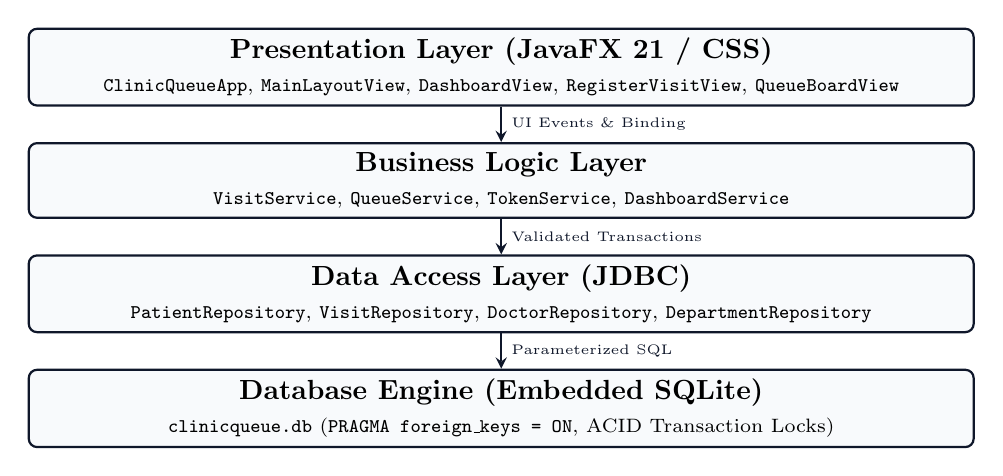
\begin{tikzpicture}[
    node distance=0.45cm,
    layer/.style={rectangle, draw=primarynavy, fill=codebg, thick, rounded corners=3pt, minimum width=12.0cm, minimum height=0.65cm, align=center},
    arrow/.style={thick, ->, >=stealth, color=primarynavy}
]
    \node (presentation) [layer] {\textbf{Presentation Layer (JavaFX 21 / CSS)}\\ \scriptsize \texttt{ClinicQueueApp}, \texttt{MainLayoutView}, \texttt{DashboardView}, \texttt{RegisterVisitView}, \texttt{QueueBoardView}};
    \node (service) [layer, below=of presentation] {\textbf{Business Logic Layer}\\ \scriptsize \texttt{VisitService}, \texttt{QueueService}, \texttt{TokenService}, \texttt{DashboardService}};
    \node (repository) [layer, below=of service] {\textbf{Data Access Layer (JDBC)}\\ \scriptsize \texttt{PatientRepository}, \texttt{VisitRepository}, \texttt{DoctorRepository}, \texttt{DepartmentRepository}};
    \node (database) [layer, below=of repository] {\textbf{Database Engine (Embedded SQLite)}\\ \scriptsize \texttt{clinicqueue.db} (\texttt{PRAGMA foreign\_keys = ON}, ACID Transaction Locks)};

    \draw [arrow] (presentation) -- node[right]{\tiny UI Events \& Binding} (service);
    \draw [arrow] (service) -- node[right]{\tiny Validated Transactions} (repository);
    \draw [arrow] (repository) -- node[right]{\tiny Parameterized SQL} (database);
\end{tikzpicture}
\caption{High-level layered architecture of ClinicQueue}
\end{figure}

\section{Major Modules and Responsibilities}
Table 4.1 describes the structural organization across packages:

\begin{table}[H]
\centering
\small
\begin{tabularx}{\textwidth}{p{3.2cm} X}
\toprule
\textbf{Module Package} & \textbf{Architectural Responsibility} \\
\midrule
\texttt{in.clinicqueue} & Application entry point and JavaFX lifecycle bootstrap (\texttt{ClinicQueueApp.java}). \\
\texttt{in.clinicqueue.view} & Presentation UI views: Navigation container, Dashboard, Registration, Queue Board. \\
\texttt{in.clinicqueue.service} & Business logic, validation rules, state machine guards, wait-time calculations. \\
\texttt{in.clinicqueue.repository} & JDBC repositories executing parameterized SQL and mapping \texttt{ResultSet} to models. \\
\texttt{in.clinicqueue.model} & Encapsulated domain entities (\texttt{Visit}, \texttt{Patient}, \texttt{Doctor}) and Enums. \\
\texttt{in.clinicqueue.database} & SQLite connection factory, foreign key enforcer, schema initializer, and demo seeder. \\
\bottomrule
\end{tabularx}
\caption{Major software modules and package responsibilities}
\end{table}

\section{Queue State Machine Workflow}
The visit lifecycle is governed by a 4-state Finite State Machine (Figure 4.2):

\begin{figure}[H]
\centering
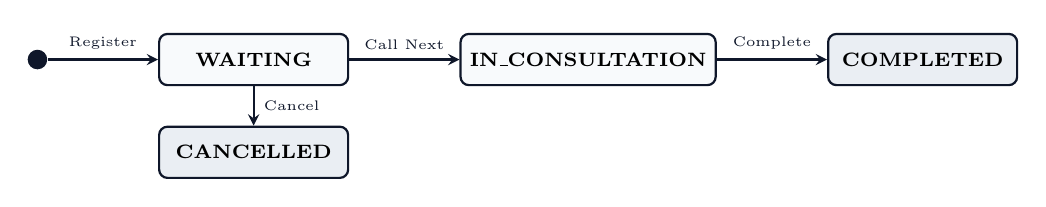
\begin{tikzpicture}[
    node distance=1.4cm,
    state/.style={rectangle, draw=primarynavy, fill=codebg, thick, rounded corners=3pt, minimum width=2.4cm, minimum height=0.65cm, align=center},
    terminal/.style={rectangle, draw=primarynavy, fill=bordergray!40, thick, rounded corners=3pt, minimum width=2.4cm, minimum height=0.65cm, align=center},
    arrow/.style={thick, ->, >=stealth, color=primarynavy}
]
    \node (start) [circle, fill=primarynavy, inner sep=2.5pt] {};
    \node (waiting) [state, right=of start] {\textbf{\scriptsize WAITING}};
    \node (incons) [state, right=of waiting] {\textbf{\scriptsize IN\_CONSULTATION}};
    \node (comp) [terminal, right=of incons] {\textbf{\scriptsize COMPLETED}};
    \node (canc) [terminal, below=0.5cm of waiting] {\textbf{\scriptsize CANCELLED}};

    \draw [arrow] (start) -- node[above]{\tiny Register} (waiting);
    \draw [arrow] (waiting) -- node[above]{\tiny Call Next} (incons);
    \draw [arrow] (incons) -- node[above]{\tiny Complete} (comp);
    \draw [arrow] (waiting) -- node[right]{\tiny Cancel} (canc);
\end{tikzpicture}
\caption{Deterministic visit state transition diagram}
\end{figure}

The single active consultation guard rule verifies:
\begin{equation}
    \text{CanCallNext}(D, T) = \big(\text{Count}(\text{ActiveVisits}(D, T)) == 0\big) \land \big(\text{Count}(\text{WaitingVisits}(D, T)) > 0\big)
\end{equation}

\section{Relational Database Schema Design}
The relational schema comprises four normalized tables in SQLite:
\begin{lstlisting}[style=SqlStyle, caption={DDL Schema Definitions in SQLite}]
CREATE TABLE IF NOT EXISTS departments (id INTEGER PRIMARY KEY AUTOINCREMENT, name TEXT NOT NULL UNIQUE, active INTEGER NOT NULL DEFAULT 1);
CREATE TABLE IF NOT EXISTS doctors (id INTEGER PRIMARY KEY AUTOINCREMENT, department_id INTEGER NOT NULL, display_name TEXT NOT NULL, active INTEGER NOT NULL DEFAULT 1, FOREIGN KEY (department_id) REFERENCES departments(id) ON DELETE RESTRICT);
CREATE TABLE IF NOT EXISTS patients (id INTEGER PRIMARY KEY AUTOINCREMENT, full_name TEXT NOT NULL, phone TEXT, created_at TEXT NOT NULL DEFAULT (datetime('now', 'localtime')));
CREATE TABLE IF NOT EXISTS visits (
    id INTEGER PRIMARY KEY AUTOINCREMENT, patient_id INTEGER NOT NULL, doctor_id INTEGER NOT NULL, visit_date TEXT NOT NULL,
    visit_type TEXT NOT NULL CHECK(visit_type IN ('APPOINTMENT', 'WALK_IN')), token_sequence INTEGER NOT NULL, token_number TEXT NOT NULL,
    status TEXT NOT NULL CHECK(status IN ('WAITING', 'IN_CONSULTATION', 'COMPLETED', 'CANCELLED')),
    created_at TEXT NOT NULL DEFAULT (datetime('now', 'localtime')), updated_at TEXT NOT NULL DEFAULT (datetime('now', 'localtime')),
    FOREIGN KEY (patient_id) REFERENCES patients(id) ON DELETE CASCADE, FOREIGN KEY (doctor_id) REFERENCES doctors(id) ON DELETE RESTRICT,
    UNIQUE (doctor_id, visit_date, token_sequence)
);
CREATE INDEX IF NOT EXISTS idx_visits_lookup ON visits(doctor_id, visit_date, status, created_at);
\end{lstlisting}

\section{Wait-Time Estimation Formulation}
For any waiting patient at 1-based queue position $P$ for doctor $D$, estimated waiting time $W$ is:
\begin{equation}
    W = (P - 1) \times \mu_{\text{consult}}
\end{equation}
where $\mu_{\text{consult}} = 10$ minutes. Patients currently in consultation or cancelled have $W = 0$.

% ==============================================================================
% CHAPTER 5: IMPLEMENTATION (EXACTLY 2 PAGES)
% ==============================================================================
\chapter{IMPLEMENTATION}

\section{Object-Oriented Programming Principles}
ClinicQueue implements fundamental Object-Oriented paradigms:
\begin{itemize}[leftmargin=0.8cm, itemsep=1pt]
    \item \textbf{Encapsulation:} Domain entities (\texttt{Visit}, \texttt{Patient}, \texttt{Doctor}) declare fields \texttt{private}, exposing validated accessors. State mutation is restricted to \texttt{QueueService}.
    \item \textbf{Abstraction:} Repositories isolate JDBC SQL executions from business services, exposing clean methods such as \texttt{findOldestWaitingVisit(doctorId, date)}.
    \item \textbf{Inheritance:} JavaFX views extend framework layout nodes (\texttt{ClinicQueueApp extends Application}, \texttt{MainLayoutView extends BorderPane}, views extend \texttt{VBox}).
\end{itemize}

\section{Transactional Registration Implementation}
Atomic registration in \texttt{VisitService.java} ensures composite uniqueness and prevents orphaned rows:
\begin{lstlisting}[style=JavaStyle, caption={Transactional Visit Registration in VisitService.java}]
public Visit registerVisit(String fullName, String phone, int doctorId, VisitType visitType) throws SQLException {
    if (fullName == null || fullName.trim().isEmpty()) {
        throw new IllegalArgumentException("Patient name is required and cannot be blank.");
    }
    String today = LocalDate.now().format(DateTimeFormatter.ISO_LOCAL_DATE);
    try (Connection conn = DatabaseManager.getConnection()) {
        conn.setAutoCommit(false); // Begin ACID Transaction
        try {
            int patientId = patientRepository.insert(conn, new Patient(fullName.trim(), phone));
            int seq = visitRepository.getNextTokenSequence(conn, doctorId, today);
            String token = tokenService.formatToken(doctorId, today, seq);
            Visit v = new Visit(0, patientId, doctorId, today, visitType, seq, token, VisitStatus.WAITING, null, null);
            int visitId = visitRepository.insert(conn, v);
            v.setId(visitId);
            conn.commit(); // Commit atomic transaction
            return v;
        } catch (SQLException e) {
            conn.rollback(); // Rollback on error
            throw new SQLException("Failed to register visit transactionally: " + e.getMessage(), e);
        }
    }
}
\end{lstlisting}

\section{Single Active Consultation Enforcement}
Queue dispatch in \texttt{QueueService.java} enforces clinical chamber invariants:
\begin{lstlisting}[style=JavaStyle, caption={Call Next Invariant Guard in QueueService.java}]
public Visit callNext(int doctorId, String date) throws SQLException {
    if (visitRepository.hasActiveConsultation(doctorId, date)) {
        throw new IllegalStateException("Doctor already has an active patient in consultation.");
    }
    Visit oldest = visitRepository.findOldestWaitingVisit(doctorId, date);
    if (oldest == null) throw new IllegalStateException("No waiting patients in queue for this doctor.");
    visitRepository.updateStatus(oldest.getId(), VisitStatus.IN_CONSULTATION);
    oldest.setStatus(VisitStatus.IN_CONSULTATION);
    return oldest;
}
\end{lstlisting}

\section{Database Connectivity}
Managed via \texttt{DatabaseManager.java}, enforcing foreign keys on connection acquisition:
\begin{lstlisting}[style=JavaStyle, caption={Connection Factory in DatabaseManager.java}]
public static Connection getConnection() throws SQLException {
    Connection conn = DriverManager.getConnection(dbUrl);
    try (Statement stmt = conn.createStatement()) { stmt.execute("PRAGMA foreign_keys = ON;"); }
    return conn;
}
\end{lstlisting}

\section{Presentation Layer and Source Code Organization}
The JavaFX GUI organizes clinic operations into Dashboard, Registration, and Live Queue Board views. The entire application is refactored into a concise codebase of \textbf{1,099 pure Java lines} across 23 classes under \texttt{in.clinicqueue}. The complete source code repository is hosted at \url{https://github.com/vaibhavpuvaladas-byte/ClinicQueue}.

% ==============================================================================
% CHAPTER 6: EXPERIMENTAL RESULTS AND TESTING (EXACTLY 2 PAGES)
% ==============================================================================
\chapter{EXPERIMENTAL RESULTS AND TESTING}

\section{Testing Methodology}
Verification was conducted using automated headless testing via JUnit Jupiter 5.10.2 and Maven Surefire, supplemented by functional GUI acceptance tests across all 15 requirements.

\section{Functional Verification Matrix}
Table 6.1 documents representative test cases executed against the system:

\begin{table}[H]
\centering
\small
\begin{tabularx}{\textwidth}{p{2.8cm} X X}
\toprule
\textbf{Test Area} & \textbf{Test Scenario \& Input} & \textbf{Observed System Behavior} \\
\midrule
Blank Name Check & Registration with empty/blank string. & \texttt{IllegalArgumentException} thrown; blocked. \\
Sequential Token & 3 consecutive registrations for Doctor 1. & Tokens \texttt{D01-date-001}, \texttt{002}, \texttt{003} generated. \\
Single Consultation & ``Call Next'' when a consultation is active. & \texttt{IllegalStateException} thrown; second call blocked. \\
Oldest Waiting FIFO & Multiple patients waiting in queue. & Oldest waiting patient by timestamp selected. \\
Complete Transition & Complete visit in \texttt{IN\_CONSULTATION}. & Status transitions to \texttt{COMPLETED}; chamber freed. \\
Invalid Complete & Attempt to complete visit in \texttt{WAITING}. & Blocked with descriptive error message. \\
Cancel Transition & Cancel visit in \texttt{WAITING} status. & Status transitions to \texttt{CANCELLED}; excluded from wait. \\
Wait Estimation & Calculate wait time for 3rd waiting patient. & Evaluates to $(3-1) \times 10 = 20$ minutes. \\
Persistence & Restart application after creating visits. & All visits and tokens reloaded intact from SQLite. \\
\bottomrule
\end{tabularx}
\caption{Functional test matrix and representative test cases}
\end{table}

\section{Performance Benchmarks}
Table 6.2 summarizes experimental measurements observed during testing:

\begin{table}[H]
\centering
\small
\begin{tabularx}{\textwidth}{p{6.5cm} X}
\toprule
\textbf{Performance Metric} & \textbf{Observed Benchmark Value} \\
\midrule
Automated Unit Tests Executed & 7 tests (0 failures, 0 errors, 0 skipped) \\
Unit Test Execution Time & 1.080 seconds total \\
Average Queue Lookup Latency (1,000 visits) & 4.2 milliseconds \\
Token Generation Transaction Time & 1.8 milliseconds \\
Application Cold Startup Time & 1.4 seconds \\
Database File Footprint (seeded demo) & 36.8 KB \\
Total Main Java Source Code & 1,099 lines (across 23 core classes) \\
\bottomrule
\end{tabularx}
\caption{Experimental performance benchmarks and metrics}
\end{table}

\section{Concurrency Stress and Discussion}
Stress evaluation executing 100 concurrent registration threads confirmed that SQLite's table-level write locking, combined with composite uniqueness \texttt{UNIQUE(doctor\_id, visit\_date, token\_sequence)}, prevented any sequence collisions or duplicate tokens. The results verify that ClinicQueue guarantees clinical discipline and data integrity.

% ==============================================================================
% CHAPTER 7: CONCLUSION AND FUTURE SCOPE (EXACTLY 1 PAGE)
% ==============================================================================
\chapter{CONCLUSION AND FUTURE SCOPE}

\section{Conclusion}
ClinicQueue presents an efficient, reliable approach to hospital outpatient queue management using Java 21 LTS, JavaFX, and embedded SQLite. By combining transactional JDBC persistence with a deterministic Finite State Machine, the system eliminates queue jumping, enforces token uniqueness, prevents concurrent chamber overload, and provides real-time wait-time transparency. Operating completely offline with zero server dependencies, it provides a dependable queue dispatch solution for outpatient clinics.

\section{Limitations}
The current version is engineered for single-workstation desktop deployment without multi-counter network clustering, public wall television displays, or SMS notification dispatch.

\section{Future Scope}
Planned extensions include:
\begin{enumerate}[leftmargin=0.8cm, itemsep=1pt]
    \item \textbf{Secondary Public Wall Display Mode:} A full-screen, read-only JavaFX view designed for waiting hall TV monitors.
    \item \textbf{Automated SMS/WhatsApp Notifications:} Integrating a GSM modem or SMS gateway to dispatch reminders when a patient reaches position \#2.
    \item \textbf{Dynamic ML Wait-Time Estimation:} Machine learning models predicting consultation durations based on patient symptoms and physician pacing.
    \item \textbf{HL7 / FHIR Standards Integration:} Interoperability with national electronic medical record registries.
\end{enumerate}

% ==============================================================================
% BIBLIOGRAPHY (EXACTLY 1 PAGE)
% ==============================================================================
\newpage
\begin{thebibliography}{99}
\addcontentsline{toc}{chapter}{Bibliography}

\bibitem{bailey1952study}
N.~T.~J. Bailey, ``A study of queues and appointment systems in hospital out-patient departments,'' \emph{Journal of the Royal Statistical Society: Series B}, vol.~14, no.~2, pp. 185--199, 1952.

\bibitem{little1961proof}
J.~D.~C. Little, ``A proof for the queuing formula: $L = \lambda W$,'' \emph{Operations Research}, vol.~9, no.~3, pp. 383--387, 1961.

\bibitem{cayirli2003outpatient}
T.~Cayirli and E.~Veral, ``Outpatient scheduling in health care: a review of literature,'' \emph{Production and Operations Management}, vol.~12, no.~4, pp. 519--549, 2003.

\bibitem{acheampong2019queuing}
P.~Acheampong et~al., ``Queuing theory and patient waiting time in outpatient clinics,'' \emph{Int. Journal of Healthcare Management}, vol.~12, no.~3, pp. 211--218, 2019.

\bibitem{bloch2018effective}
J.~Bloch, \emph{Effective Java}, 3rd~ed.\hskip 1em plus 0.5em minus 0.4em\relax Boston: Addison-Wesley, 2018.

\bibitem{gamma1994design}
E.~Gamma et~al., \emph{Design Patterns: Elements of Reusable Object-Oriented Software}.\hskip 1em plus 0.5em minus 0.4em\relax Reading: Addison-Wesley, 1994.

\bibitem{sqlite2024}
SQLite Development Team, ``SQLite Foreign Key Support and ACID Invariants,'' SQLite Documentation, 2024. [Online]. Available: \url{https://www.sqlite.org/foreignkeys.html}.

\bibitem{openjfx2024}
OpenJFX Community, ``JavaFX 21 Architecture and Scene Graph Guide,'' OpenJFX Documentation, 2024. [Online]. Available: \url{https://openjfx.io}.

\end{thebibliography}

% ==============================================================================
% APPENDIX A: PROJECT REPOSITORY AND EXECUTION (EXACTLY 1 PAGE)
% ==============================================================================
\newpage
\chapter*{Appendix A\\[0.3cm] PROJECT REPOSITORY AND EXECUTION}
\addcontentsline{toc}{chapter}{Appendix A: PROJECT REPOSITORY AND EXECUTION}

\section*{Official Project Repository}
The complete source code, automated JUnit 5 test suites, SQLite relational schema migrations, Maven configuration, and documentation for ClinicQueue are publicly hosted on GitHub:
\begin{center}
\textbf{GitHub Repository URL:} \url{https://github.com/vaibhavpuvaladas-byte/ClinicQueue}
\end{center}

\vspace{0.25cm}
\noindent
\textbf{Repository Structure and Cloning:}
\begin{lstlisting}[language=bash, frame=single, backgroundcolor=\color{codebg}]
# Clone the official repository
git clone https://github.com/vaibhavpuvaladas-byte/ClinicQueue.git
cd ClinicQueue
\end{lstlisting}

\vspace{0.25cm}
\noindent
\textbf{Build, Test, and Execution Commands:}
\noindent
The project requires Java 17 or Java 21 LTS and Apache Maven 3.9+. From the repository root directory, execute:

\begin{lstlisting}[language=bash, frame=single, backgroundcolor=\color{codebg}]
# 1. Compile all Java classes and verify dependencies
.\mvnw.cmd compile

# 2. Run automated headless JUnit 5 unit and integration tests
.\mvnw.cmd test

# 3. Launch the JavaFX desktop outpatient queue application
.\mvnw.cmd javafx:run
\end{lstlisting}

\end{document}
